\chapter{muEDM positron tracker}
\begin{refsection}
{\itshape This chapter is an in-depth study on the development of the scintillating fiber part of the muEDM positron tracker. 
We will skip the preliminary studies and we will start with the description of the positron tracker which was included in the proposal of the experiment submitted to PSI at the end of 2022; we will move to the simulations done after that and the current design of this detector.}
\section{Proposal}
\subsection{SciFi prototype}
The detector described in the proposal would satisfy the requirements for muEDM but comes with some limitations and some oversight.
\subsection{The barrel geometry}
\subsection{Issues}
\subsection{Alternatives}

\section{CHeT or CyFi}
The first step in developing and prototyping the geometry chosen in the previous paragraph is to understand the requirements for this sub-detector and how the prospected resolutions compare to these.
This scintillating fiber tracker will be used for position tracking and in particular is going to be complemented by silicon strips. The crucial information this system needs to provide is the longitudinal position of the particle with a good resolution: $\delta \ell \lesssim \SI{1}{mm}$.

\subsection{Resoutions of crossed fibers ribbons}
Let's consider a ribbon  $\SI{3}{cm}\times\SI{15}{cm}$ of squared fibers \SI{250}{\micro m} running vertically. Assuming a `perfect' readout, the resolution across the ribbon is given simply by the fibers' width while the resolution along the ribbon is extracted by reading the fibers on both sides. This second resolution is often quite worse than the previous. For practical purposes we will here assume $\delta_x = \SI{1}{mm};\ \delta_y = \SI{10}{mm}$.
Rotating the ribbon by an angle $\theta$ changes the projection of the resolutions on the $\hat{x};\ \hat{y}$ axes and for this reason crossing two ribbons can improve the resolutions on the position of a crossing particle.
\noindent
When reading the ribbon on both sides the resolutions, as a function of $\theta$, are given by the smaller between the projection of the two intrinsic resolutions.  
\begin{equation}
    \begin{cases}
      \dd x = min(\delta x \sec \theta;\ \delta y \csc \theta)\\
      \dd y = min(\delta x \csc \theta;\ \delta y \sec \theta)
    \end{cases}
\end{equation}
The relation between resolutions and the tilt angle is shown in fig. \ref{fig:CyFi:projected_dxdy}.  

\begin{figure}
    \centering
    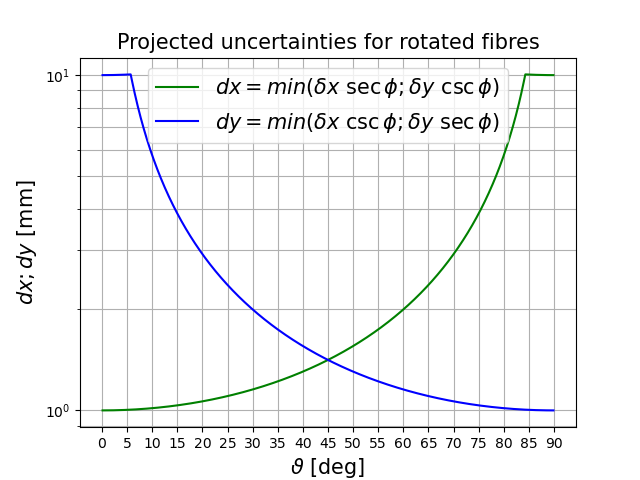
\includegraphics[width=\textwidth]{Figures/muEDM/CyFi/projected_dxdy.png}
    \caption{Projection along the $\hat{x};\ \hat{y}$ axes of the resolutions considering a ribbon of fibers rotated in different angles. The intrinsic resolutions are here assumed $\delta_x = \SI{1}{mm};\ \delta_y = \SI{10}{mm}$.}
    \label{fig:CyFi:projected_dxdy}
\end{figure}


\subsection{Angle choices for the layers}
When considering two layers the angles must be chosen to improve the overall resolution, which in practice means minimizing the uncertainty only on one axes per ribbon.
Let's consider the different layouts in \ref{fig:CyFi:examples:a} and how they translate to resolutions in \ref{fig:CyFi:examples:b}.
Clearly having the two ribbons at \SI{90}{\deg} along the axes is the best option but if we want to avoid having the readout on the plane of the muon orbit we need to consider less steep angles for the single ribbons.
Options C and D are the possible solutions and, looking at the resolutions, D is actually the configuration minimizing the resolutions on both axes. 

\noindent
At this point is important to notice an additional constraint, given by the cylindrical geometry: if two fibers cross multiple times when both are scintillating the position of the impinging particle is ill-defined. There is a `real' crossing point but also additional `ghosts' hits.
If we consider a two-layer system the requirement of having only one crossing point (i.d. no `ghosts') translates to having a difference in the number of turns $\lesssim1$. 
In a cylindrical geometry the relation between the angle of the fibers and the number of turns completed, shown in Fig.~\ref{fig:CyFi:TurnsVsAngles}, is determined by the dimensions of the cylinder itself.
At this point, we can plot the resolutions as a function of the angle of one of the layers keeping the angle for the second layer such as $\Delta T=0$. The results are in Fig.~\ref{fig:CyFi:projected_dxdy} while Fig.~\ref{fig:CyFi:angle} shows the difference in angle for the two layers.
We will consider two concentric cylinders, the outer layer being the one with a shallower angle: this is intended to reduce the effect of multiple scattering on the longitudinal position.

\begin{figure}
\subfloat[Some possible orientation for two ribbons.]{
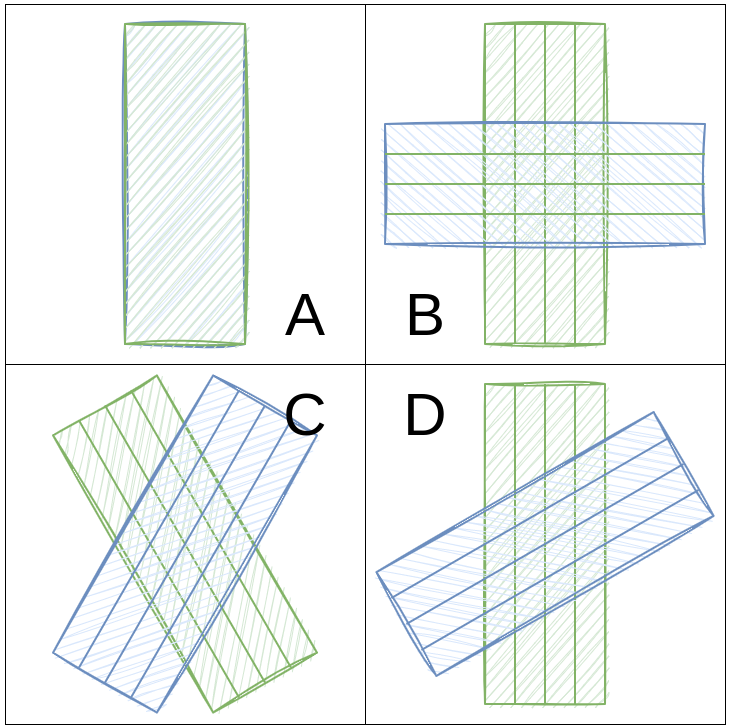
\includegraphics[width=0.41\textwidth, keepaspectratio]{Figures/muEDM/CyFi/CrossingFibres_config.png}
\label{fig:CyFi:examples:a}}
\subfloat[Projected uncertainties as a function of the outer layer's angle]{
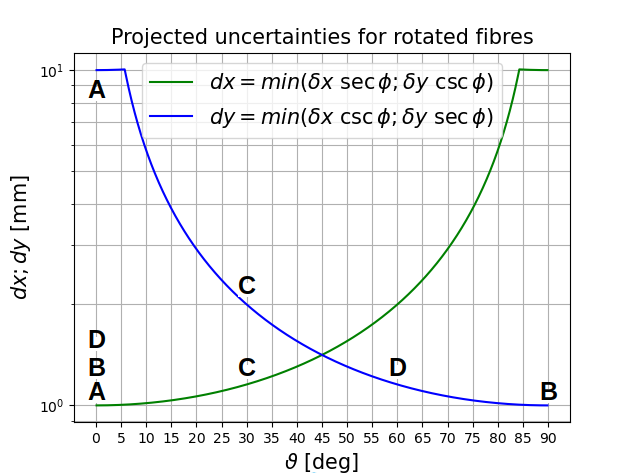
\includegraphics[width=0.57\textwidth, keepaspectratio]{Figures/muEDM/CyFi/projected_dxdy_examples.png}
\label{fig:CyFi:examples:b}}
\caption{Relation between the direction of the fibers and the associated uncertainties projected onto the axes. Some specific orientations of two overlapping ribbons are shown.}
\end{figure}

\begin{figure}
    \centering
    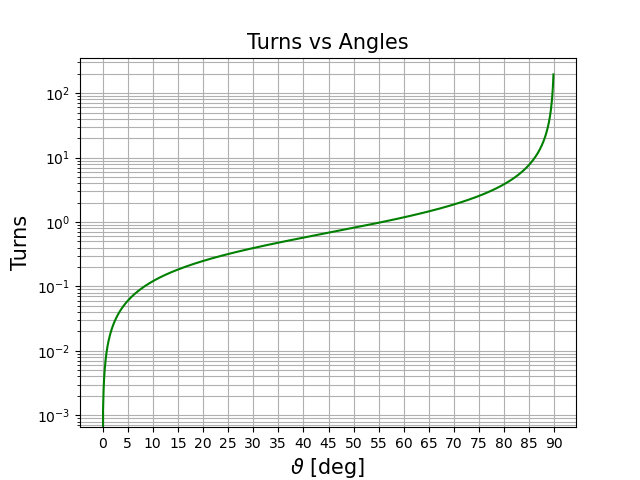
\includegraphics[width=\textwidth]{Figures/muEDM/CyFi/TurnsVsAngles.png}
    \caption{In a planar configuration, the angle at which the fibers run translates directly to the angle at which the ribbon is oriented. In a cylindrical geometry a fiber running at a given angle will complete different number of turns depending on the dimensions of the cylinder.}
    \label{fig:CyFi:TurnsVsAngles}
\end{figure}


\begin{figure}[ht]   
\centering
\subfloat[Projected uncertainties as a function of the outer layer's angle]{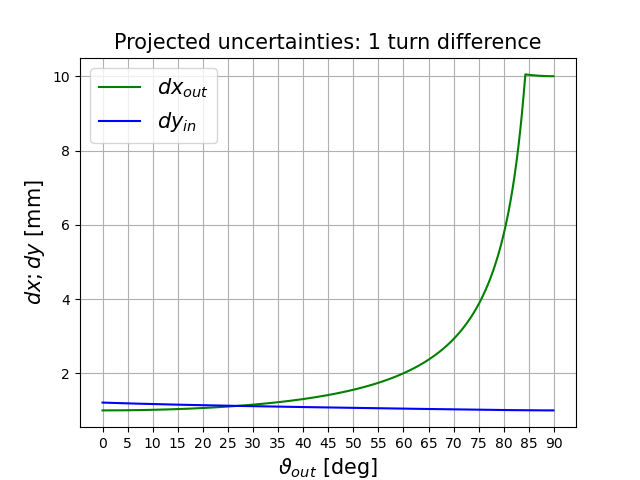
\includegraphics[width=0.49\textwidth, keepaspectratio]{Figures/muEDM/CyFi/projected_dxdy_1Turn.png}\label{fig:CyFi:projected_dxdy}}
\hfill
\subfloat[Angle of the inner layer and difference in angle as a function of the angle of the outer layer]{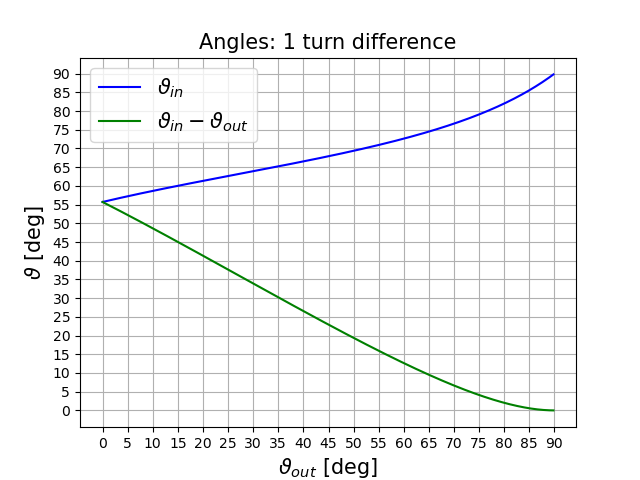
\includegraphics[width=0.49\textwidth, keepaspectratio]{Figures/muEDM/CyFi/Angles_1Turn.png}\label{fig:CyFi:angle}}
\caption{The results when considering two layers in a cylindrical geometry keeping the requirement $\Delta T=0$: \ref{fig:CyFi:projected_dxdy} shows the projected uncertainties; \ref{fig:CyFi:angle} shows the angle of the inner layer.}
\label{fig:CyFi}
\end{figure}

Building the layers with infinite precision on the angle is clearly not feasible for this reason we can use the plots in Fig.~\ref{fig:CyFi:5deg}, where the angles have been rounded to multiples of \SI{5}{\deg}. 
Additional attention we can have is to consider the length of the scintillating fibers: if the fibers are too long the light collection at the ends is decreased by the absorption. The length of the fibers in both layers is shown as a function of the outer angle in Fig.~\ref{fig:CyFi:5deg:length}.
Clearly, this is the extreme case: depending on the intrinsic resolutions of the fibers, shallower angles and $\Delta T<1$ could be chosen, simplifying the construction. 
\begin{figure}[ht]   
\centering
\subfloat[Angle of the inner layer and difference in angle as a function of the angle of the outer layer]{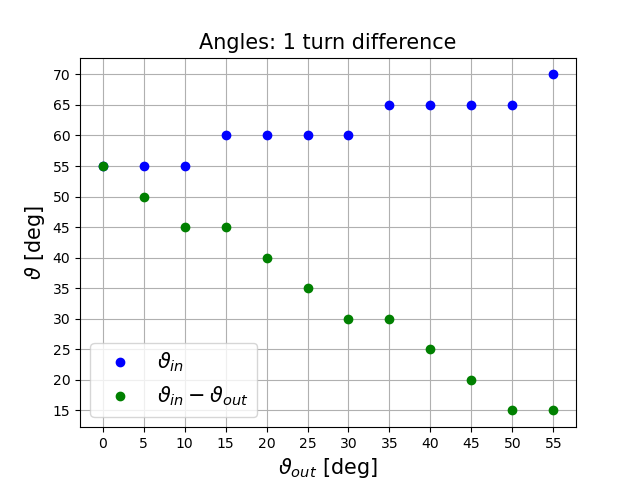
\includegraphics[width=0.49\textwidth, keepaspectratio]{Figures/muEDM/CyFi/Angles_1Turn_60deg_5deg.png}\label{fig:CyFi:5deg:angle}}
\hfill
\subfloat[Projected uncertainties as a function of the outer layer's angle]{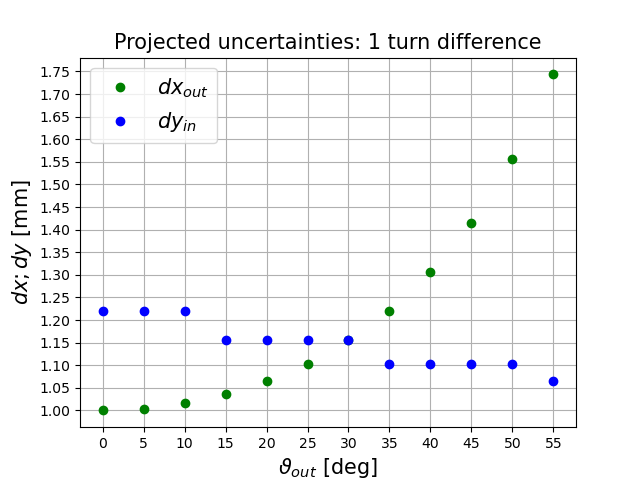
\includegraphics[width=0.49\textwidth, keepaspectratio]{Figures/muEDM/CyFi/projected_dxdy_1Turn_60deg_5deg.png}\label{fig:CyFi:5deg:projected_dxdy}}\\
\subfloat[Fibers' length as a function of the outer layer's angle]{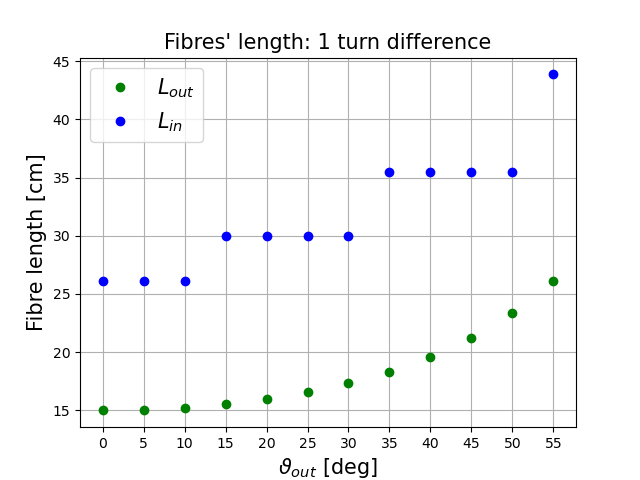
\includegraphics[width=0.49\textwidth, keepaspectratio]{Figures/muEDM/CyFi/FibreLength_1Turn_60deg_5deg.png}\label{fig:CyFi:5deg:length}}
\caption{Key parameters as a function of the outer layer's angle keeping 1 turn difference between the two layers and rounding the angles to multiples of \SI{5}{\deg}.}
\label{fig:CyFi:5deg}
\end{figure}



\subsection{Geant4 simulation}
\paragraph{G4TessellatedSolid} The first hurdle in the Geant4 simulation for this sub-detector is the definition of the geometry. 
The shape is the result of wrapping a squared fiber around a cylinder resulting in a `squared helix'.
After some consideration there are two ways of defying this geometry:
\begin{outline}
    \1 Taking bool difference of two G4TwistedBox\footnote{The documentation can be found here: \href{https://apc.u-paris.fr/~franco/g4doxy/html/classG4TwistedBox.html}{G4TwistedBox}}. 
    This is a simple solution but comes with some limitations: the shape of the fiber cannot be changed to circular; the twisted box cannot be twisted more than \SI{90}{\deg}, so a stack of clones is needed; 
    \1 Defying the geometry using G4TessellatedSolid\footnote{The documentation can be found here: \href{https://apc.u-paris.fr/~franco/g4doxy/html/classG4TessellatedSolid.html}{G4TessellatedSolid}}, which means creating it by hand triangulating the shape. Clearly, this is a more cumbersome solution but it allows for more flexibility.
\end{outline}
The core part of the code for generating the G4TessellatedSolid fibers is in appendix \ref{ch:G4TessellatedSolid}.

\paragraph{Fibers and read-out} Aside from the specific geometry, cardinal point is how to describe the fibers and their readout. 
The fiber itself is simulated as a three layer volume:
\begin{outline}
    \1 Core: 
    \1 First cladding: PMMA
    \1 Second cladding: PMMA EMA
\end{outline}
The optical property of the surface between the different layers is specified with a G4OpticalSurface\footnote{The documentation can be found here: \href{https://apc.u-paris.fr/~franco/g4doxy/html/classG4OpticalSurface.html}{G4OpticalSurface}}.
The readout simulates a SiPM:
\begin{outline}
    \1 Optical grease: 
    \1 SiPM window: Silicon resin
    \1 SiPM :
\end{outline}

\subsection{From photons to waveforms}
The simulation in \gf ends with the recording of the optical photons entering the SiPM SensitiveDetectors.
The physical processes going from the impinging photons to the analog signal are quite complex and simulating them would require a lot of effort (and CPU time).
To get a feeling of the type of signals we can expect from the simulation we can create a simple script \textit{faking} the readout.
The required steps are:
\begin{outline}
    \1 \textit{PDF}: probability of a photon converting. 
    This is a binomial distribution and is SiPM dependent: reasonable values $p_{PDF}\in [0.3, 0.5]$
    \1 \textit{Response}: per photon converted, add a 'waveform' at the photon time. 
    The shape $w(t)$ is SiPM/electronics dependent but some assumptions can be made.
    \1 \textit{Dark noise}: add a probability of spurious photons converting. 
    This is a poissonian process that gives $n_{dark}$ photons distributed flat in the readout time.
\end{outline}

\begin{equation}
    W(t)=\sum_{i=0}^{n_\gamma} w(t_i)\cdot p_{PDF} + \sum_{i=0}^{n_{dark}} w(t_{flat})
\end{equation}

Once we obtain $W(t)$ we can apply a threshold $th$ and turn the signal from analog to digital. 
If the \textit{th} is crossed, we recorded a \textit{hit}.
Clearly, given the geometry under consideration, we need two \textit{hits} to make a \textit{chit}.
Mapping pairs of hits in chits is not trivial and takes as parameters the dimensions of the cylinder and the SiPM numbers (or alternatively the their position).

\subsection{From \textit{hits} to \textit{c-hits}}

\section{Prototype/Beamtime}

\section{Conclusions}

\addcontentsline{toc}{chapter}{Bibliography on muEDM positron tracker}
\printbibliography[title=Bibliography on muEDM positron tracker]
\end{refsection}